\documentclass[10pt, AMS Euler]{article}
\textheight=9.25in \textwidth=7in \topmargin=-.75in
\oddsidemargin=-0.25in
\evensidemargin=-0.25in
\usepackage{url}  % The bib file uses this
\usepackage{graphicx} %to import pictures
\usepackage{amsmath, amssymb}
\usepackage{theorem, concrete, multicol, color}


\setlength{\intextsep}{5mm} \setlength{\textfloatsep}{5mm}
\setlength{\floatsep}{5mm}


{\theorembodyfont{\rmfamily}
	\newtheorem{definition}{Definition}[section]}
{\theorembodyfont{\rmfamily} \newtheorem{example}{Example}[section]}
{\theorembodyfont{\rmfamily} \newtheorem{lemma}{Lemma}[section]}
{\theorembodyfont{\rmfamily} \newtheorem{theorem}{Theorem}[section]}
{\theorembodyfont{\rmfamily} \newenvironment{proof}{\par{\it
			Proof:}}{\nopagebreak[4]\rule{2mm}{2mm}}}


%%%%  SHORTCUT COMMANDS  %%%%
\newcommand{\ds}{\displaystyle}
\newcommand{\Z}{\mathbb{Z}}
\newcommand{\arc}{\rightarrow}
\newcommand{\R}{\mathbb{R}}
\newcommand{\N}{\mathbb{N}}
\newcommand{\Q}{\mathbb{Q}}
\newcommand{\stirling}[2]{\genfrac{\{}{\}}{0pt}{}{#1}{#2}}

%%%%  footnote style %%%%

\renewcommand{\thefootnote}{\fnsymbol{footnote}}

\pagestyle{empty}
\begin{document}
	
	\noindent{\bf \large MATH 3310 -- Midterm Experience} \\
	Fall 2026\\
	David E Brown\\
	
	\noindent {\bf Constraints:} You may discuss the problems below with the following set of people: 
	\begin{eqnarray*} P &=& \{\mbox{Anyone currently enrolled in MATH 3310}, \\ 
		&& \mbox{David Brown, Mcrae Arnold, Gideon Walker}\}.\end{eqnarray*}
	
	The only resources we may use to solve the problems posed in this experience are our brains.  The use of anything beyond that is cheating. 
	
	The solutions to this Experience should be created by groups of at most four and are to be submitted October 31, 2026,  by 11:59pm.
	
	
	\vspace{2em}
	
	\noindent \maltese \hspace{1ex} {\bf Sub-Experience One: \emph{Pizza Cutting with Lasers}}\\
	
	\noindent **No outside resources, please** 
	Given the difficulty of organizing and sequentially lining up cuts to get the maximum number of pieces, you invent a laser cutting system that allows you to make all cuts at once.  
	You place $n$ of your devices on the crust with spacing that will maximize the number of pieces made and, once activated (ideally remotely because they are dangerous), \emph{laser sabers}$^{\circledR}$ shoot between every pair of devices simultaneously cutting the pizza into $R(n)$ pieces\footnote{``$R$'' for lase\underline{R}.}.  
	Below is an illustration representing $5$ of your devices cutting the pizza into $16$ pieces.  
	
	\begin{center}
		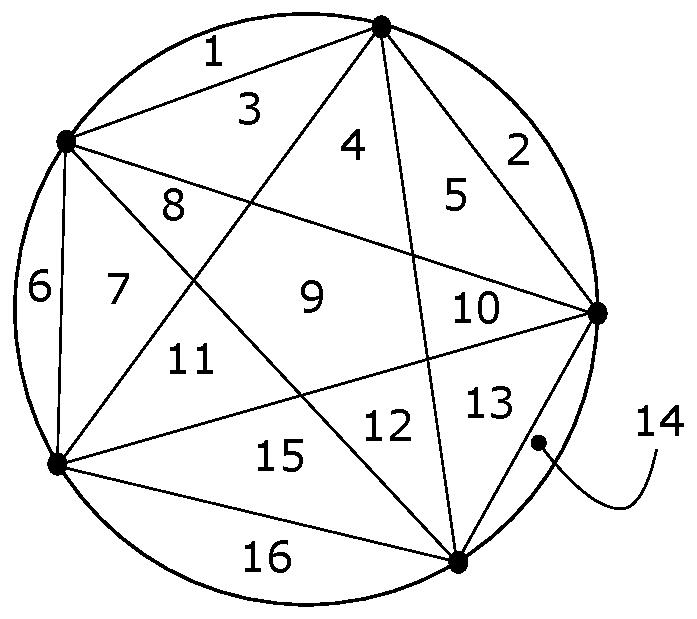
\includegraphics[scale=0.5]{5pointsOnCircleEx}
	\end{center}
	
	\noindent Please determine a formula for $R(n)$.  

	{\bf Answer:}
	\bigskip
	To begin we decided to gather data to see how we could determine the relationship. We drew the pizza slices out with different numbers of nodes on our papers and gathered the following data:

	\begin{center}
		\begin{tabular}{l|ccccccccccc}\hline
			
			{\bf $n$ } & 0 & 1 & 2 & 3 & 4 & 5 & 6 & 7 \\
			\hline \hline
			{\bf $P(n)$} & 1 & 1 & 2 & 4 & 8 & 16 & 31 & 57  \\
		\end{tabular}
	\end{center}

	\bigskip
	\noindent One issue we saw while drawing out the different pizza diagrams is that it was easy to draw three points intersecting eachother. Since we are trying to maximize the number of slices we instead offset the nodes to avoid intersections of more then two lines. This helps us to maximize the number of pieces. 

	\bigskip
	\noindent We decided to use the calculus method to solve this problem. To start we created a difference table as pictured below. It pictures the first through fifth difference of $P(n)$.  

	\begin{center}
			\begin{tabular}{l|ccccccccccc}\hline
				
				{\bf $n$ } & 0 & 1 & 2 & 3 & 4 & 5 & 6 & 7 \\
				\hline \hline
				{\bf $P(n)$} & 1 & 1 & 2 & 4 & 8 & 16 & 31 & 57  \\
				$\Delta P(n)$ & 0 & 1 & 2 & 4 & 8 & 15 & 26 &   \\
				$\Delta^2P(n)$  & 1 & 1 & 2 & 4 & 7 & 11 &  &    \\
				$\Delta^3P(n)$  & 0  &  1  & 2 & 3 & 4 & &  &   \\
				$\Delta^4P(n)$  & 1  &  1  & 1 & 1 &  & &  &   \\
				$\Delta^5P(n)$  & 0  &  0  & 0 &  &  & &  &   \\
			\end{tabular}
		\end{center}
	
	\vspace{1em}

	\noindent Based on the fact that $\delta^5P(n)$ is all zeroes we can assume that the equation $P(n)$ may be represented by a equation of this form: 
	
	\bigskip
	$P(n) = An^4 +Bn^3 +Cn^2 + Dn + E$

	\bigskip
	\noindent To solve for the coefficents $A, B, C, D, E$ we want to create a system of equations we could use to solve for them. We use the data we gathered above to create a system of equations which is pictured below. 


	\bigskip
	\[
	\begin{bmatrix}
	0 & 0 & 0 & 0 & 1 \\
	1 & 1 & 1 & 1 & 1 \\
	16 & 8 & 4 & 2 & 1 \\
	81 & 27 & 9 & 3 & 1 \\
	256 & 64 & 16 & 4 & 1
	\end{bmatrix}
	\begin{bmatrix}
	A \\
	B \\
	C \\
	D \\
	E
	\end{bmatrix}
	=
	\begin{bmatrix}
	1 \\
	1 \\
	2 \\
	4 \\
	8
	\end{bmatrix}
	\]

	\bigskip
	\noindent We plugged this equation into a matrix calculator to solve for the coefficents. We got the following results.

	\bigskip
	\[
	\begin{bmatrix}
	A \\
	B \\
	C \\
	D \\
	E
	\end{bmatrix}
	=
	\begin{bmatrix}
	0.041667 \\
	-0.250000 \\
	0.958333 \\
	-0.750000 \\
	1.000000
	\end{bmatrix}
	\]

	\bigskip
	\noindent We can plug these into our initial equation for the final equation:

	\bigskip
	$P(n) = 0.041667n^4 - .25n^3 + .95833 n^2 - .75 n + 1$

	\bigskip
	\noindent We tested this by plugging in all the values of n we had manually calculated, and found that this equation described our function for all values from $ n = 0$ to $n = 7$

	\bigskip
	\noindent As we had more answers then we needed to solve the system of equations we are assuming that this equation has been proven and is correct. 
	
	\noindent \underline{\hspace{5in}}
	
	\vspace{2em}
	
	\noindent \maltese \hspace{1ex} {\bf Sub-Experience Two: \emph{Strange Walks}}\\
	
	After the pizza, you decide to take a walk.\\
	
	\noindent {\bf Number of shortest paths using the \emph{city block metric}}.  
	Starting at Center and Main, you decide to walk to $X$ North and $Y$ East.
	The distance is measured in blocks and so the distance from $X_1$ North and $Y_1$ East to $X_2$ North and $Y_2$ East is $|X_2 - X_1| + |Y_2 - Y_1|$. \\
	
	\noindent{\bf SE 2.1.} For yuks, determine $\pi$ in the Logan metric.  
	Use the fact that $\pi$ is defined to be the ratio of the circumference to the diameter of a circle, and that a circle is the set of points equidistant from a given point (that distance is typically called the \emph{radius} of the circle and the point is called its \emph{center}).  
	Remember that, in this context, `\emph{distance}' has been redefined.  

	\bigskip
	\noindent

	{\bf Answer:}
	In this context we are using the logan metric, so the way we measure distance has changed. When we create a circle (A set of points equidistant from a given center) it ends up creating a diamond shape. This is pictured in the image below. 

	\begin{center}
		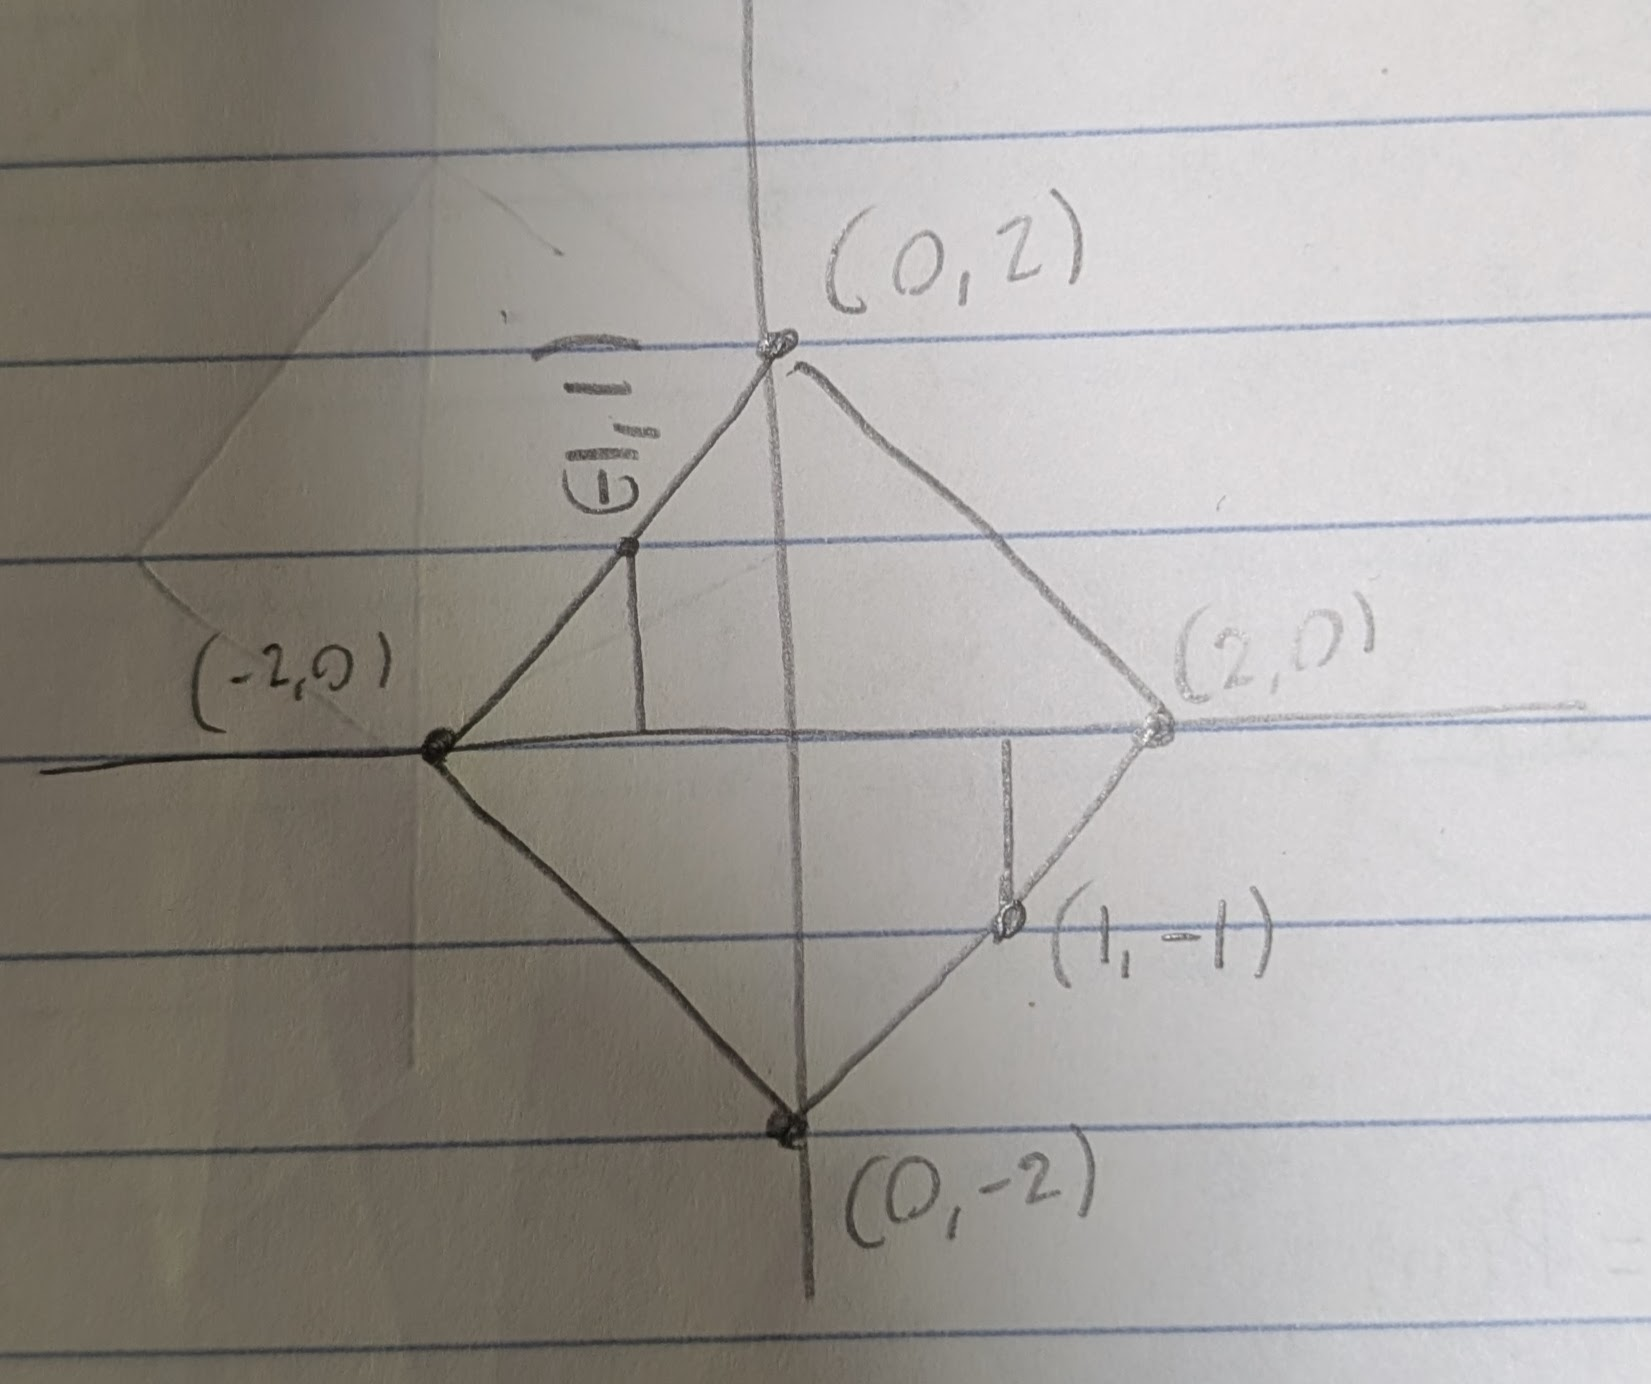
\includegraphics[scale=0.2]{circle_diamond.jpg}
	\end{center}

	\bigskip
	\noindent
	The equation relating circumference to the diameter of a circle is 

	\bigskip
	\noindent
	$C = \pi * D$

	\bigskip
	\noindent
	Where $D = Diameter$ and $C = Circumference$

	\bigskip
	\noindent

	To solve for $\pi$ we need a circumference and diameter that correspond to eachother.  Lets use a "circle" of diameter 4. This is what we used to create the diamond pictured above. To solve for $\pi$ we need to find the circumference of a "circle" of diameter 4. 
	
	\bigskip
	\noindent

	Using pythagoreams theorem we can find that the length of each of the individual sides of the diameter 4 diamond is equal to $\sqrt(2*R^2)$ where R is our radius. We have four sides so the circumference is equal to $4 * \sqrt(2R^2)$

	\bigskip
	\noindent

	Now knowing both the circumference and the diameter we can plug these values in and solve for $\pi$

	\bigskip
	\noindent

	$\pi = (4 * \sqrt(2 * 2^2))\div(4)$

\bigskip
	\noindent

	$\pi = (2*\sqrt(2))$

\bigskip
	\noindent

	This is the final answer for this problem. 
	
\bigskip
	\noindent
	
	\noindent{\bf SE 2.2.}  Count the number of shortest paths from Center and Main to $X$ North and $Y$ East.  A more erudite way to pose this problem is as follows: count paths from $(0,0)$ to $(X,Y)$ using steps of the form $R: (x,y) \mapsto (x+1,y)$ or $U:(x,y) \mapsto (x,y+1)$.  So paths trace rectilinear ``curves'' in the first quadrant of the Cartesian coordinate system that visit only integer-valued coordinates. \\
	
	\vspace{1em}
	
	\noindent{\bf SE 2.3.}  Walk in a strange way.  Start at Center and Main, thinking of it as the origin $(0,0)$ and take $n$ steps, each of type $R$, $L$, or $U$, with $R$ never followed by $L$ and vice-versa. The steps are defined via $R:(x,y) \mapsto (x+1,y)$, $L:(x,y) \mapsto (x-1,y)$, and $U:(x,y) \mapsto (x, y+1)$.  
	Determine the number of different paths with $n$ steps.
	
	\noindent{\bf SE 2.4.}  Given what happens when you take the red pill, you choose the blue one ... and turn into a puma ...  and find yourself in the Yucatan peninsula at the base of a Mayan temple.  Whoa.  
	You find that your puma strength allows you to clear one or two terraces in a single bound.  
	For reasons known only by the metaphysics of the blue pill, you need to 
	
	\begin{enumerate}
		\item Compute $P_n$, the number of ways to ascend an 
		$n$-terraced temple. Please determine $P_n$ by finding a recurrence relation and then using the recurrence relation find a closed formula for $P_n$.  
		Calculate $P_{365}$ because the temple you're facing has $365$ terraces.
		
		\item Again, for reasons which clear only to you as you are under the influence of the blue pill, you must prove that 
		$$P_n = \sum_{i=0}^{\lfloor n/2 \rfloor}\binom{n-i}{i}.$$
	\end{enumerate}
	
	
	\begin{center}
		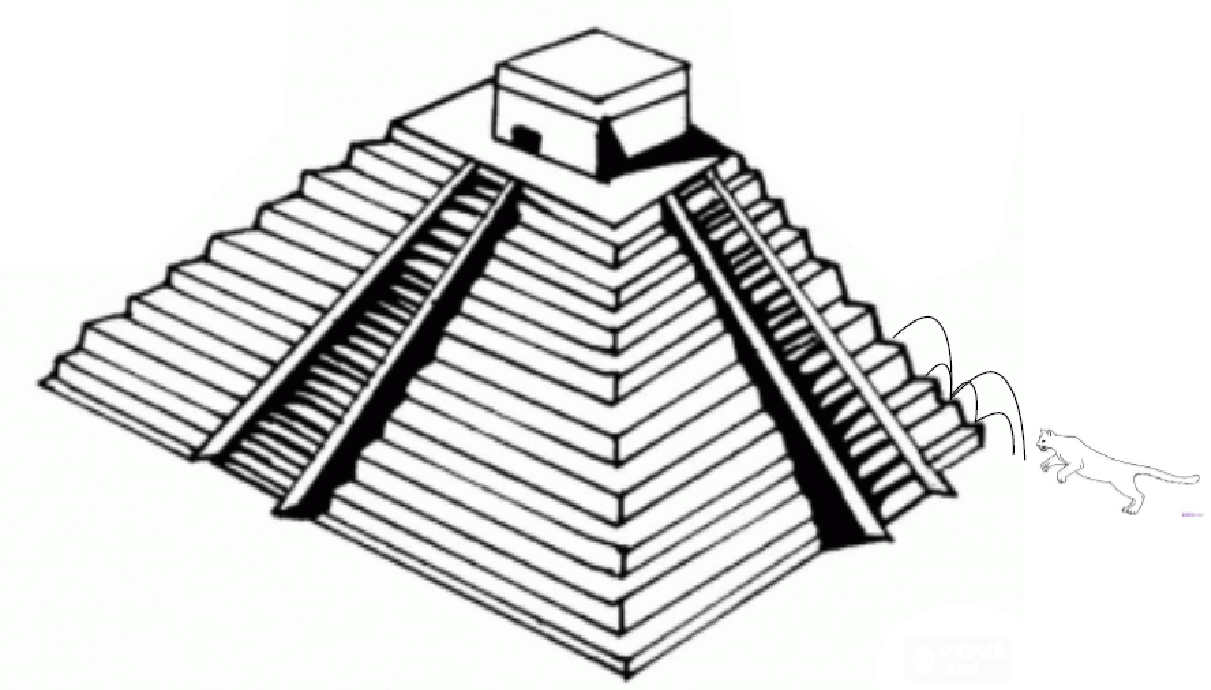
\includegraphics[scale=0.4]{Puma_and_temple}
	\end{center}
	
	
	
	\vspace{1em}
	
	\noindent \underline{\hspace{5in}}
	
	
	\vspace{2em}
	
	\noindent \maltese \hspace{1ex}{\bf Sub-Experience Three: The Master Table of Distributions.} \\
	
	\noindent  Below is the table of distribution functions $f:A \to B$, where $A$ is a finite set with $n$ elements and $B$ is a finite set with $x$ elements.  
	The goal: determine a formula for the number of functions with properties described by the table for each of the twelve possibilities.  
	So, for example, the entry in cell 5 of the table is to be the number of injective functions that map a set of $n$ indistinguishable object into a set of $x$ distinguishable objects. 
	
	$$\begin{array}{c|c||c|c|c}
		\hline A & B & \mbox{unrestricted }& \mbox{injective}& \mbox{onto} \\ \hline \hline
		\mbox{distinguishable} & \mbox{distinguishable} & 1. & 2. & 3. \\ \hline
		\mbox{indistinguishable}& \mbox{distinguishable}&4.&5.&6. \\ \hline
		\mbox{distinguishable} & \mbox{indistinguishable}& 7. & 8. & 9. \\ \hline
		\mbox{indistinguishable}&\mbox{indistinguishable}& 10. &11.&12. \\ \hline \end{array}$$\\

		1. $x^n$
		2. 
		3. 
		4.
		5. $ \binom{x}{n}$ 
		6.  
		7. $\begin{cases} 
  			1 & \text{if } x = 1 \\ 
  			xk & \text{if } 1 < x < n \\ 
  			x! & \text{if } x \geq n  
			\end{cases}$ 
		8. $1$ 
		9. 
		10. $P(n)$ 
		11. $1$ 
		12. $P_x(n)$ 
	
	\noindent Please determine, with an argument for each, a formula for each entry in the table.\\
	
	\vspace{1em}
	
	\noindent \underline{\hspace{5in}}
	
	\vspace{2em}
	
	
	
	\noindent \maltese \hspace{1ex} {\bf Sub-Experience Four: \emph{Game Time!}}\\
	
	\noindent{\bf SE 4.1: Modified Towers of Hanoi.}  The \emph{Towers of Hanoi} are mythical diamond needles, three of them, with $64$ gold discs impaled on one of the needles.  God told the monks of Brahma to transfer all the discs to another needle with the constraints that no larger disc ever be placed atop a smaller disc, and only one disc at a time is to be moved.  Once the monks finish moving the discs the World will end.  Evidently the monks have not yet finished. \\    
	
	\noindent Label the needles of the Towers of Hanoi $L$, $M$,
	and $R$, for the left, middle, and right, respectively.  
	Consider the original Towers of Hanoi game,
	but with the additional constraint that a disk can only be moved to an adjacent peg; that is, a disk can only be moved to $M$ from $L$ or $R$, and can only be moved to $L$ or $R$ from $M$.  
	Assume all discs are initially on $L$. \\
	
	\noindent \emph{Determine the minimum number of moves (where a \emph{move} is defined to be the transfer of one disc from one needle to another) required to transfer $n$ discs from $L$ to $R$.}\\

	\bigskip
	\noindent

	{\bf Answer:}
	We started by manually computing the number of moves required to move each of the individual discs from the L needle to the R needle. We ran these calculations up to N = 6. We were able to find the number of moves required to move from the L needle to the R needle for the number of n pins using the chart below.

	\bigskip
	\noindent
	In this chart the uppermost row tells us how many discs we are trying to move. The next rows tell us how many times each discs had to be moved in order to move all discs from L to R. For example, when we are moving 2 discs, we had to move disc 1 4 times and disc 2 2 times. 

	\begin{center}
		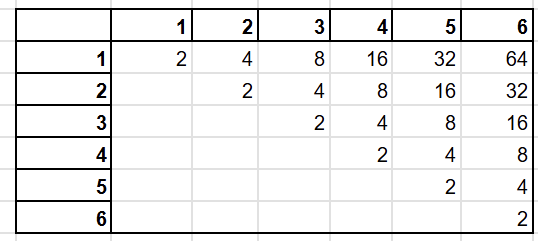
\includegraphics[scale=1]{Hanoi.png}
	\end{center}

	\bigskip
	\noindent
	This chart revealed a pattern that to move N discs there is a summation we can use. By observation I was able to see the following sum we can use to represent how many moves it takes to move N discs. 

	\bigskip
	\noindent
	$\sum_{k=1}^{n} \sum_{w=1}^{k} 2^w $

	\bigskip

	
	\noindent \emph{How Long?} Assume the monks of Brahma were given this game with $64$ discs, and can move a disc at a rate of one per second. How long in centuries will it take for the monks to complete their task?\\

	\bigskip
	\noindent

	{\bf Answer:}
	Next we want to see how long it would take the monks to move 64 discs if each move takes 1 second. We can input $n = 64$ into the equation above which tells us we will need approximately $7.3786976295\times10^{19}$ seconds, which is equal to $4.737994774\times10^{17}$ centuries. A very long time. 
	
	\vspace{1em}
	
	
	\noindent {\bf SE 4.2: A Two-Player Game with no Dire Consequences.} \\
	
	\noindent{\bf The Game}\\
	
	\noindent Two players, $A$ and $B$, alternately select an \emph{edge} (line segment connecting two dots) on the grid graph shown 
	below and color it red.
	The loser of the game is the player who is forced to select an edge that creates
	a red $C_4$ --- a red cycle on $4$ vertices.\\
	
	\begin{center}
		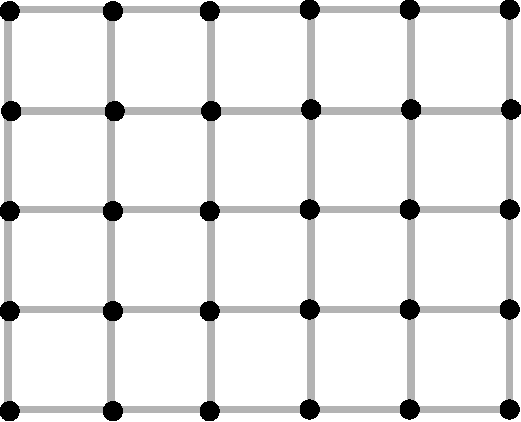
\includegraphics[scale=0.5]{Saturator_Grid}
	\end{center}
	
	\noindent{\bf The Fun}\\
	
	\noindent \emph{Confirm or deny, with proof, whether player $A$ (the first player) can always 
		win if she employs a particular strategy for each move.}
	
	\vspace{1em}
	
	\noindent \underline{\hspace{5in}}
	
	\vspace{2em}
	
	\noindent \maltese \hspace{1em} {\bf Sub-Experience Five -- A Matter of Life and Death}\\
	
	\noindent **No outside resources**  You are among a group of $n-1$  of your friends (pretend you have $n-1$ friends even if you don't, where $n$ is possibly very large)
	and are captured by a horde of theater students who will force you and your $n-1$ friends to
	enact the play \emph{Cats} with them over and over and over and ... .  
	Your friends choose death over this fate and decide to
	form a circle and have every other person commit suicide (someone has a pistol and $n$ bullets,
	which is quite reasonable to assume here at USU) until only one person survives, who will
	supposedly kill themselves.  
	You want no part of this suicide madness since, you figure, the theater people will tire eventually and
	you can make your escape by taking Jennyanydots hostage with the pistol and remaining bullet and escape.\\
	
	\noindent Number you and your friends $1$ to $n$ and assume you all form a vicious circle to facilitate the suicide.\\
	
	\noindent \textsf{Question:} \emph{In which position (call it $S(n)$) must you be in order to survive?}\\
	
	\noindent Examples: $S(4) =1$, $S(7) =7$.
	
	\vspace{1em}
	
	\noindent \underline{\hspace{5in}}
	
	
	
\end{document}